% !TEX root = ../main.tex
\documentclass[../main.tex]{subfiles}

\begin{document}

\chapter{Power and Agency in Intermediary Discourse}
\labch{power}
\margintoc

\begin{quote}
\textit{``Language is a powerful medium that intricately encodes social dynamics between people, such as perspectives, biases, and power differentials.''}\\
--- Antoniak et al. \cite{antoniak2023riveter}
\end{quote}

\section{Introduction: Who Does What to Whom in Innovation Ecosystems?}[Introduction]
\labsec{power:intro}

How do innovation intermediaries linguistically construct power relations among ecosystem actors?\marginnote{Power relations in innovation ecosystems shape resource allocation, decision-making authority, and whose voices are heard in sustainability transitions \cite{avelino2017power}.} When the EIT describes how ``Climate-KIC \textit{accelerates} startups'' or how ``entrepreneurs \textit{transform} industries,'' these verb choices encode implicit claims about who holds power, who exercises agency, and who is acted upon. Such linguistic framings are not neutral descriptions but active constructions that shape how stakeholders understand their roles within innovation ecosystems.

This chapter applies verb-based connotation frame analysis to examine power and agency dynamics in EIT KIC communications.\sidenote{Connotation frames capture the implied social dynamics encoded in verb predicates---who has power over whom, who exercises agency, and how actors are valued \cite{rashkin2016connotation,sap2017connotation}.} Building on the RIVETER framework \cite{antoniak2023riveter}, we extract Agent-Verb-Theme triples from EIT discourse to measure how different actors---entrepreneurs, researchers, corporations, policymakers, and the KICs themselves---are positioned in power hierarchies and attributed agency. Our analysis addresses three chapter-level research questions contributing to \textbf{RQ3} on discursive roles:

\begin{enumerate}
    \item \textbf{CRQ1}: How are different actor types positioned in terms of power and agency in EIT discourse?
    \item \textbf{CRQ2}: How do power and agency framings vary across KICs?
    \item \textbf{CRQ3}: What verb patterns characterize high-power versus low-power actor positions?
\end{enumerate}

Our findings reveal systematic asymmetries. Institutional actors---the EIT itself, the European Commission, and specific KICs---are consistently framed with high agency and power; actor categories like ``Startups'' and ``Partners'' carry negative power scores and more frequently appear as objects of institutional action than as autonomous agents. ``Partners'' show a particularly striking pattern: high agency (0.621) combined with negative power ($-0.224$)---active but subordinate. These patterns persist across all eight KICs with moderate variation, suggesting a shared institutional discourse template.

\begin{center}
\small
\begin{tabular}{lrrrr}
\toprule
\textbf{KIC} & \textbf{Documents} & \textbf{Sentences} & \textbf{Relations} & \textbf{Avg. Rels/Doc} \\
\midrule
EIT Central & 385 & 7,564 & 2,588 & 6.7 \\
InnoEnergy & 194 & 4,923 & 1,635 & 8.4 \\
Climate-KIC & 131 & 2,934 & 862 & 6.6 \\
EIT Digital & 125 & 3,371 & 932 & 7.5 \\
EIT Health & 92 & 2,219 & 667 & 7.2 \\
RawMaterials & 82 & 2,388 & 720 & 8.8 \\
EIT Food & 64 & 1,571 & 443 & 6.9 \\
Urban Mobility & 26 & 508 & 95 & 3.7 \\
Manufacturing & 22 & 553 & 194 & 8.8 \\
Unclassified & 152 & 5,161 & 1,587 & 10.4 \\
\midrule
\textbf{Total} & \textbf{1,273} & \textbf{31,192} & \textbf{9,723} & \textbf{7.6} \\
\bottomrule
\end{tabular}
\captionof{table}{Overview of corpus and quality-filtered verb-entity relations.
From 23,781 raw extracted triples, a three-stage quality pipeline removed pronouns and noise tokens (4,599), non-entity actors via NER whitelist validation (9,459), yielding 9,723 clean relations across 795 unique verbs.
Expanded lexicon covers 100\% of corpus verbs (2,354 lexicon entries).}
\labtab{corpus-overview-power}
\end{center}

\section{Methods: Connotation Frame Analysis}[Methods]
\labsec{power:methods}

% ── Workflow Schematic ──────────────────────────────────────────────────────
\begin{wideblock}
\centering
\begin{tikzpicture}[
    scale=0.78, transform shape,
    stepbox/.style={draw, rounded corners=3pt, fill=#1!15,
        minimum width=2.6cm, minimum height=1.5cm,
        align=center, font=\scriptsize, inner sep=4pt},
    uibox/.style={draw, rounded corners=3pt, fill=CoverGold!25,
        minimum width=2.6cm, minimum height=1.5cm,
        align=center, font=\scriptsize, inner sep=4pt,
        line width=1pt},
    ethicslabel/.style={font=\fontsize{5.5}{6.5}\selectfont,
        text=AccentCoral!80!black, align=center, text width=2.4cm},
    arrow/.style={->, thick, PandaCharcoal!60},
]
    % ── Pipeline steps ──
    \node[stepbox=Azure] (s1) at (0,0)
        {\faNewspaper\\[0.15em]\textbf{News Corpus}\\[0.1em]1,273 articles};
    \node[stepbox=AccentCyan] (s2) at (3.2,0)
        {\faTag\\[0.15em]\textbf{NER + Gazetteer}\\[0.1em]spaCy + custom};
    \node[stepbox=AccentCyan] (s3) at (6.4,0)
        {\faCogs\\[0.15em]\textbf{RIVETER Pipeline}\\[0.1em]23,781 $\to$ 9,723};
    \node[stepbox=AccentPurple] (s4) at (9.6,0)
        {\faBook\\[0.15em]\textbf{Lexicon Scoring}\\[0.1em]2,354 annotated verbs};
    \node[stepbox=PandaBamboo] (s5) at (12.8,0)
        {\faUserShield\\[0.15em]\textbf{Entity Profiling}\\[0.1em]813 entities scored};
    \node[uibox] (ui) at (16,0)
        {\faDesktop\\[0.15em]\textbf{RIVETER-X}\\[0.1em]Interactive UI};

    % ── Arrows ──
    \draw[arrow] (s1) -- (s2);
    \draw[arrow] (s2) -- (s3);
    \draw[arrow] (s3) -- (s4);
    \draw[arrow] (s4) -- (s5);
    \draw[arrow] (s5) -- (ui);

    % ── Ethics annotations ──
    \node[ethicslabel] at (0,-1.3)
        {\faBalanceScale~Source bias:\\EIT-centric coverage};
    \node[ethicslabel] at (3.2,-1.3)
        {\faBalanceScale~NER errors:\\entity misclassification};
    \node[ethicslabel] at (6.4,-1.3)
        {\faBalanceScale~Quality filtering:\\59\% triples removed};
    \node[ethicslabel] at (9.6,-1.3)
        {\faBalanceScale~Lexicon bias:\\English connotations};
    \node[ethicslabel] at (12.8,-1.3)
        {\faBalanceScale~Score reification:\\aggregation effects};
    \node[ethicslabel] at (16,-1.3)
        {\faLockOpen~Open source:\\full transparency};
\end{tikzpicture}
\captionof{figure}{Analytical workflow for power and agency analysis. Ethical considerations (coral) annotate each step. The pipeline flows from news corpus through named entity recognition, RIVETER verb-connotation extraction, lexicon scoring, and entity profiling. The \textsc{Riveter-X} UI enables interactive exploration of power dynamics.}
\label{fig:ch9:workflow}
\end{wideblock}

\subsection{Connotation Frames and the RIVETER Pipeline}

For any verb predicate $v$ with Agent $a$ and Theme $t$, connotation frames \cite{rashkin2016connotation} capture implied social dynamics---effect, value, and perspective---beyond denotational meaning.\marginnote{Frame semantics argues that understanding a sentence involves knowledge evoked by concepts in the sentence, not just denotational meaning \cite{fillmore1976frame}.} \textcite{sap2017connotation} extended this with \textit{power} (the differential between Agent and Theme) and \textit{agency} (whether the Agent is decisive and can act upon their environment) dimensions. When someone ``\textit{accelerates}'' another, the Agent has power over the Theme and high agency; when someone ``\textit{receives},'' the Agent has low power and low agency.

% Figure 9.1: Connotation frame dimensions
\begin{center}
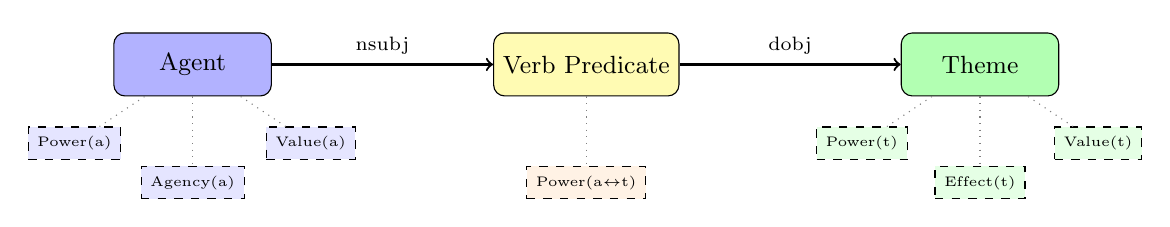
\begin{tikzpicture}[
    node/.style={rectangle, draw, rounded corners, minimum width=2cm, minimum height=0.8cm, font=\small},
    arrow/.style={->, thick},
]
% Verb predicate center
\node[node, fill=yellow!30] (verb) at (5, 2) {Verb Predicate};

% Agent
\node[node, fill=blue!30] (agent) at (0, 2) {Agent};

% Theme
\node[node, fill=green!30] (theme) at (10, 2) {Theme};

% Arrows
\draw[arrow] (agent) -- (verb) node[midway, above, font=\scriptsize] {nsubj};
\draw[arrow] (verb) -- (theme) node[midway, above, font=\scriptsize] {dobj};

% Connotation dimensions - Agent side
\node[draw, dashed, fill=blue!10, font=\tiny] (agency) at (0, 0.5) {Agency(a)};
\node[draw, dashed, fill=blue!10, font=\tiny] (powera) at (-1.5, 1) {Power(a)};
\node[draw, dashed, fill=blue!10, font=\tiny] (valuea) at (1.5, 1) {Value(a)};

% Connotation dimensions - Theme side
\node[draw, dashed, fill=green!10, font=\tiny] (powert) at (8.5, 1) {Power(t)};
\node[draw, dashed, fill=green!10, font=\tiny] (valuet) at (11.5, 1) {Value(t)};
\node[draw, dashed, fill=green!10, font=\tiny] (effectt) at (10, 0.5) {Effect(t)};

% Relational dimension
\node[draw, dashed, fill=orange!10, font=\tiny] (persp) at (5, 0.5) {Power(a$\leftrightarrow$t)};

% Connections
\draw[gray, dotted] (agent) -- (agency);
\draw[gray, dotted] (agent) -- (powera);
\draw[gray, dotted] (agent) -- (valuea);
\draw[gray, dotted] (theme) -- (powert);
\draw[gray, dotted] (theme) -- (valuet);
\draw[gray, dotted] (theme) -- (effectt);
\draw[gray, dotted] (verb) -- (persp);

\end{tikzpicture}
\captionof{figure}{Connotation frame dimensions for verb predicates (adapted from \cite{sap2017connotation})}
\labfig{connotation-frame}
\end{center}

\marginnote{%
\scriptsize
\begin{tabular}{lcc}
\toprule
\textbf{Verb} & \textbf{Agency(a)} & \textbf{Power(a$\leftrightarrow$t)} \\
\midrule
accelerate & + & + \\
transform & + & + \\
enable & + & = \\
support & + & + \\
empower & + & $-$ \\
benefit & = & $-$ \\
receive & $-$ & $-$ \\
depend & $-$ & $-$ \\
\bottomrule
\end{tabular}\\[2pt]
Example verb connotations
% \labtab{verb-examples}
}

We adapt the RIVETER framework \cite{antoniak2023riveter} for EIT discourse analysis through six stages: document parsing (spaCy), entity recognition (NER + custom gazetteer for actor categories), coreference resolution (fastcoref; \cite{otmazgin2023lingmess}), Agent-Verb-Theme triple extraction via dependency parsing, entity quality filtering (pronoun removal, NER whitelist validation, name normalization), and lexicon matching.\sidenote{The full pipeline architecture is described in \cref{ch:method}; validation details are in the replication box at the end of this chapter.} The expanded lexicon combines \textcite{sap2017connotation}'s power/agency annotations (2,148 verbs) with transition-specific and buildup/breakdown dimensions, yielding 2,354 annotated verbs with 100\% coverage of the 795 unique corpus verbs.

\subsection{Corpus and Actor Categories}

The corpus comprises 1,273 documents (31,192 sentences) from EIT KIC public communications spanning 2015--2024, emphasizing strategic and promotional content where power framing is most salient (\cref{tab:corpus-overview-power}).\sidenote{Technical reports and financial documents were excluded.} Raw triple extraction yielded 23,781 Agent-Verb-Theme relations; after quality filtering, 9,723 clean relations remained. LLM-based entity type classification further filtered 112 noise artifacts, yielding 813 meaningful entity profiles across 10 semantic types.\sidenote{Entity types: Concept (193), Actor Type (178), Organization (177), Person (139), Program (32), Institution (29), Technology (23), Event (22), GPE (12), Location (8).}

For each entity $e$, we aggregate connotation scores across all triples where $e$ appears as Agent or Theme, computing mean agency and power scores with bootstrap confidence intervals (1,000 resamples).

\section{Findings: Power and Agency in EIT Discourse}[Findings]
\labsec{power:findings}

\subsection{Overall Actor Positioning}

\cref{fig:actor-scores} presents mean power and agency scores for key entities across the full corpus, distinguishing institutional actors, actor categories, and geopolitical references.

% Figure 9.3: Power and agency scores by entity
\begin{center}
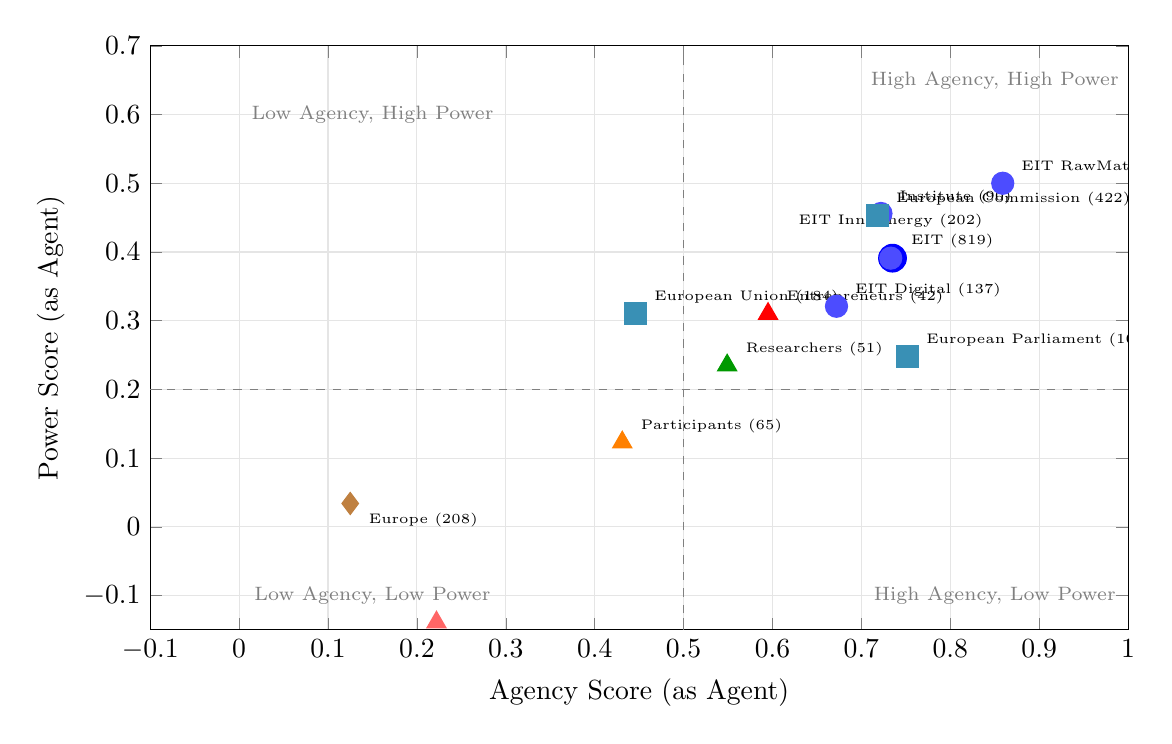
\begin{tikzpicture}
\begin{axis}[
    width=14cm,
    height=9cm,
    xlabel={Agency Score (as Agent)},
    ylabel={Power Score (as Agent)},
    xmin=-0.1, xmax=1.0,
    ymin=-0.15, ymax=0.7,
    grid=major,
    grid style={gray!20},
]

% Institutional actors (blue markers)
\addplot[only marks, mark=*, mark size=5pt, blue] coordinates {(0.735, 0.391)}; % EIT
\addplot[only marks, mark=*, mark size=4pt, blue!70] coordinates {(0.859, 0.500)}; % EIT RawMaterials
\addplot[only marks, mark=*, mark size=4pt, blue!70] coordinates {(0.733, 0.391)}; % EIT InnoEnergy
\addplot[only marks, mark=*, mark size=4pt, blue!70] coordinates {(0.672, 0.321)}; % EIT Digital
\addplot[only marks, mark=*, mark size=4pt, blue!70] coordinates {(0.722, 0.456)}; % Institute

% Policymakers (cyan markers)
\addplot[only marks, mark=square*, mark size=4pt, cyan!70!black] coordinates {(0.718, 0.453)}; % European Commission
\addplot[only marks, mark=square*, mark size=4pt, cyan!70!black] coordinates {(0.446, 0.310)}; % European Union
\addplot[only marks, mark=square*, mark size=4pt, cyan!70!black] coordinates {(0.752, 0.248)}; % European Parliament

% Actor categories (warm markers)
\addplot[only marks, mark=triangle*, mark size=4pt, red] coordinates {(0.595, 0.310)}; % Entrepreneurs
\addplot[only marks, mark=triangle*, mark size=4pt, red!60] coordinates {(0.222, -0.139)}; % Startups
\addplot[only marks, mark=triangle*, mark size=4pt, green!60!black] coordinates {(0.549, 0.235)}; % Researchers
\addplot[only marks, mark=triangle*, mark size=4pt, orange] coordinates {(0.431, 0.123)}; % Participants
\addplot[only marks, mark=diamond*, mark size=4pt, purple] coordinates {(0.621, -0.224)}; % Partners
\addplot[only marks, mark=diamond*, mark size=4pt, brown] coordinates {(0.125, 0.034)}; % Europe

% Labels
\node[font=\tiny, anchor=south west] at (axis cs:0.745, 0.391) {EIT (819)};
\node[font=\tiny, anchor=south west] at (axis cs:0.869, 0.500) {EIT RawMaterials (64)};
\node[font=\tiny, anchor=south] at (axis cs:0.733, 0.420) {EIT InnoEnergy (202)};
\node[font=\tiny, anchor=south west] at (axis cs:0.682, 0.321) {EIT Digital (137)};
\node[font=\tiny, anchor=south west] at (axis cs:0.732, 0.456) {Institute (90)};
\node[font=\tiny, anchor=south west] at (axis cs:0.728, 0.453) {European Commission (422)};
\node[font=\tiny, anchor=south west] at (axis cs:0.456, 0.310) {European Union (184)};
\node[font=\tiny, anchor=south west] at (axis cs:0.762, 0.248) {European Parliament (105)};
\node[font=\tiny, anchor=south west] at (axis cs:0.605, 0.310) {Entrepreneurs (42)};
\node[font=\tiny, anchor=north west] at (axis cs:0.232, -0.139) {Startups (36)};
\node[font=\tiny, anchor=south west] at (axis cs:0.559, 0.235) {Researchers (51)};
\node[font=\tiny, anchor=south west] at (axis cs:0.441, 0.123) {Participants (65)};
\node[font=\tiny, anchor=south west] at (axis cs:0.631, -0.224) {Partners (58)};
\node[font=\tiny, anchor=north west] at (axis cs:0.135, 0.034) {Europe (208)};

% Quadrant labels
\node[font=\scriptsize, gray] at (axis cs:0.85, -0.10) {High Agency, Low Power};
\node[font=\scriptsize, gray] at (axis cs:0.15, 0.60) {Low Agency, High Power};
\node[font=\scriptsize, gray] at (axis cs:0.85, 0.65) {High Agency, High Power};
\node[font=\scriptsize, gray] at (axis cs:0.15, -0.10) {Low Agency, Low Power};

% Reference lines at median
\draw[gray, dashed] (axis cs:0.5, -0.15) -- (axis cs:0.5, 0.7);
\draw[gray, dashed] (axis cs:-0.1, 0.2) -- (axis cs:1.0, 0.2);

\end{axis}
\end{tikzpicture}
\captionof{figure}{Mean power and agency scores for key entities (as Agent). Circles: institutional actors; squares: policymakers; triangles: actor categories; diamonds: other. Numbers in parentheses indicate mentions after quality filtering ($n$=9,723 relations).}
\labfig{actor-scores}
\end{center}

\subsubsection{High Power/High Agency: The Innovation Protagonists}

Institutional actors---EIT, the European Commission, and specific KICs---cluster in the high-power, high-agency quadrant.\marginnote{These institutional actors are constructed as the protagonists of innovation narratives---those who act upon the world and exercise power over others.} EIT alone accounts for 819 mentions, appearing as Agent in 95.8\% of cases. The verbs most frequently carrying high power scores encode decisive action and provision:

\begin{center}
\small
\begin{tabular}{lrr}
\toprule
\textbf{Verb} & \textbf{Count} & \textbf{Power(a)} \\
\midrule
publish & 200 & +1 \\
develop & 183 & +1 \\
provide & 155 & +1 \\
add & 126 & +1 \\
launch & 122 & +1 \\
offer & 106 & +1 \\
make & 96 & +1 \\
use & 75 & +1 \\
propose & 75 & +1 \\
lead & 69 & +1 \\
bring & 67 & +1 \\
create & 65 & +1 \\
\bottomrule
\end{tabular}
\captionof{table}{Most Frequent High-Power Verbs in Corpus (Power(a) = +1)}
\labtab{high-power-verbs}
\end{center}

Institutional actors ``\textit{publish},'' ``\textit{develop},'' and ``\textit{provide}''---verbs positioning them as powerful producers and distributors of resources. They ``\textit{launch}'' and ``\textit{create}''---verbs encoding decisive capability. These actors are rarely positioned as Themes: EIT appears as Agent in 95.8\% of its mentions; the European Commission in 97.4\% of 422 mentions.

\subsubsection{Low Power/Low Agency: The Beneficiaries}

Actor categories like ``people'' and ``entrepreneurs'' occupy positions with markedly lower power and agency.\sidenote{These actor categories are constructed as objects of institutional action rather than agents in their own right---recipients of support delivered by KICs and policymakers.} The most frequent low-power verbs encode need, reception, and dependency:

\begin{center}
\small
\begin{tabular}{lrr}
\toprule
\textbf{Verb} & \textbf{Count} & \textbf{Power(a)} \\
\midrule
announce & 126 & $-1$ \\
receive & 126 & $-1$ \\
need & 92 & $-1$ \\
explain & 80 & $-1$ \\
join & 75 & $-1$ \\
want & 72 & $-1$ \\
become & 62 & $-1$ \\
call & 42 & $-1$ \\
represent & 38 & $-1$ \\
believe & 32 & $-1$ \\
recognise & 31 & $-1$ \\
benefit & 30 & $-1$ \\
\bottomrule
\end{tabular}
\captionof{table}{Most Frequent Low-Power Verbs in Corpus (Power(a) = $-1$)}
\labtab{low-power-verbs}
\end{center}

\marginnote{%
\scriptsize
\begin{tabular}{lrr}
\toprule
\textbf{Entity} & \textbf{Agent} & \textbf{Theme} \\
\midrule
EIT & 95.8\% & 4.2\% \\
Eur. Commission & 97.4\% & 2.6\% \\
EIT InnoEnergy & 93.6\% & 6.4\% \\
Institute & 98.9\% & 1.1\% \\
Researchers & 92.2\% & 7.8\% \\
Entrepreneurs & 76.2\% & 23.8\% \\
Partners & 74.1\% & 25.9\% \\
Startups & 77.8\% & 22.2\% \\
\bottomrule
\end{tabular}\\[2pt]
Agent vs.\ Theme position by entity
% \labtab{agent-theme-ratio}
}

``Startups'' appear as Themes (22.2\% of 36 mentions) far more often than institutional actors, and with negative power ($-0.139$). ``Partners'' show the starkest contrast: high agency (0.621) but negative power ($-0.224$), appearing as Themes in 25.9\% of cases---active but subordinate. ``Researchers'' (power: 0.235, agency: 0.549, $n$=51) and ``Participants'' (power: 0.123, agency: 0.431, $n$=65) occupy intermediate positions with moderate agency but lower power.\marginnote{Researchers are constructed as having expertise (moderate agency) but not as exercising power over others---an important asymmetry relative to institutional actors.}

\subsection{Cross-KIC Variation}

% Figure 9.4: Agency, power, and buildup scores by KIC
\begin{center}
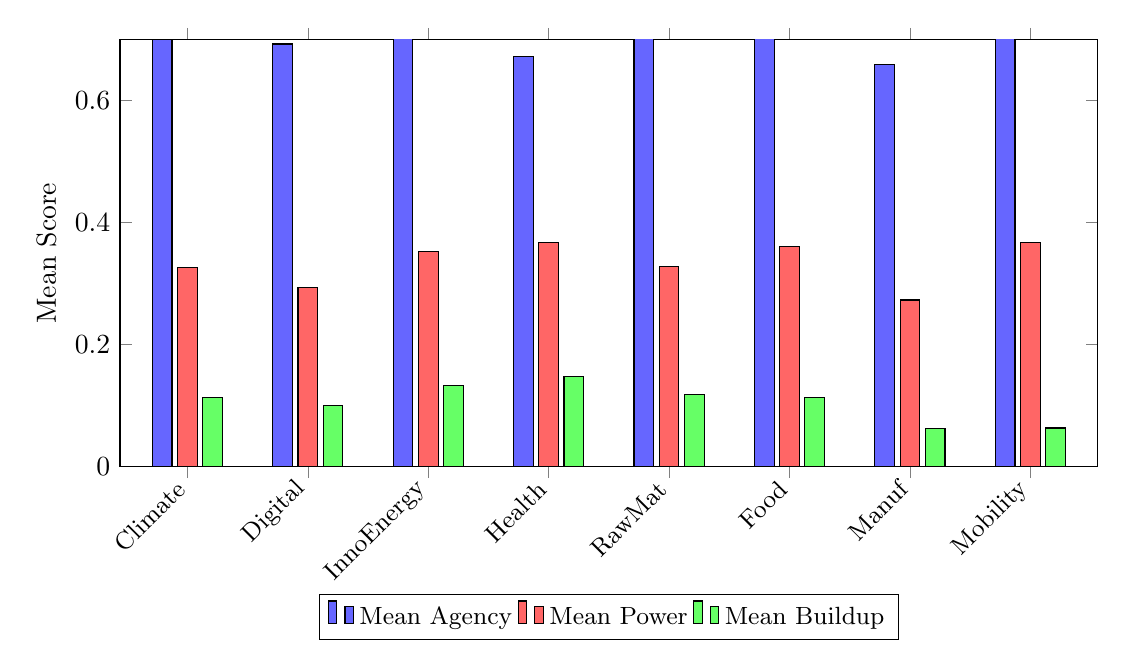
\begin{tikzpicture}
\begin{axis}[
    ybar,
    width=14cm,
    height=7cm,
    ylabel={Mean Score},
    symbolic x coords={Climate, Digital, InnoEnergy, Health, RawMat, Food, Manuf, Mobility},
    xtick=data,
    x tick label style={rotate=45, anchor=east, font=\small},
    ymin=0, ymax=0.7,
    legend style={at={(0.5,-0.3)}, anchor=north, legend columns=3, font=\small},
    bar width=0.25cm,
    enlarge x limits=0.08,
]

% Agency scores
\addplot[fill=blue!60] coordinates {
    (Climate, 0.700)
    (Digital, 0.693)
    (InnoEnergy, 0.750)
    (Health, 0.672)
    (RawMat, 0.725)
    (Food, 0.756)
    (Manuf, 0.660)
    (Mobility, 0.747)
};

% Power scores
\addplot[fill=red!60] coordinates {
    (Climate, 0.326)
    (Digital, 0.294)
    (InnoEnergy, 0.352)
    (Health, 0.367)
    (RawMat, 0.328)
    (Food, 0.361)
    (Manuf, 0.273)
    (Mobility, 0.368)
};

% Buildup scores
\addplot[fill=green!60] coordinates {
    (Climate, 0.113)
    (Digital, 0.100)
    (InnoEnergy, 0.133)
    (Health, 0.148)
    (RawMat, 0.118)
    (Food, 0.113)
    (Manuf, 0.062)
    (Mobility, 0.063)
};

\legend{Mean Agency, Mean Power, Mean Buildup}

\end{axis}
\end{tikzpicture}
\captionof{figure}{Mean agency, power, and buildup scores by KIC (all relations within KIC-attributed documents)}
\labfig{kic-comparison}
\end{center}

EIT Urban Mobility (mean power: 0.368), EIT Health (0.367), and EIT Food (0.361) show the highest power scores, reflecting discourse that frames institutional actors as decisive authorities directing resource flows.\sidenote{Health discourse emphasises institutional authority over clinical and regulatory processes; food and mobility discourse position KICs as powerful coordinators of complex supply chains and urban systems.} EIT Food (agency: 0.756) and InnoEnergy (0.750) show the highest agency scores, reflecting discourse emphasizing transformation and system change.\marginnote{EIT Health shows the highest buildup score (0.148), followed by InnoEnergy (0.133), reflecting constructive framing around building new infrastructure.}

Comparing across all eight KICs reveals moderately homogeneous power scores (range: 0.273--0.368) with somewhat wider variation in agency (0.660--0.756).\sidenote{The modest cross-KIC power variation suggests a shared institutional discourse template, with sectoral differences manifesting primarily in agency and buildup framing.} The most notable variation appears in buildup scores: EIT Health (0.148), InnoEnergy (0.133), and RawMaterials (0.118) show the highest constructive framing, while Manufacturing (0.062) and Urban Mobility (0.063) show the lowest---the two newest KICs, possibly reflecting still-emerging institutional identities.

\subsection{Verb Pattern Analysis}

% Figure 9.5: Verb frequency heatmap by actor
\begin{center}
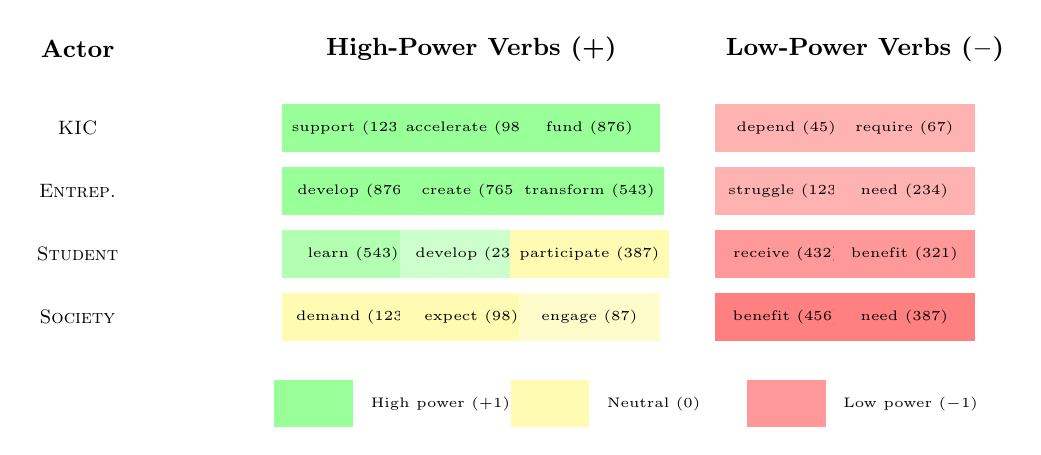
\begin{tikzpicture}[
    cell/.style={minimum width=1.8cm, minimum height=0.6cm, font=\tiny, align=center},
]

% Headers
\node[font=\small\bfseries] at (0, 4) {Actor};
\node[font=\small\bfseries] at (5, 4) {High-Power Verbs (+)};
\node[font=\small\bfseries] at (10, 4) {Low-Power Verbs ($-$)};

% KIC row
\node[font=\scriptsize] at (0, 3) {\textsc{KIC}};
\node[cell, fill=green!40] at (3.5, 3) {support (1234)};
\node[cell, fill=green!40] at (5, 3) {accelerate (987)};
\node[cell, fill=green!40] at (6.5, 3) {fund (876)};
\node[cell, fill=red!30] at (9, 3) {depend (45)};
\node[cell, fill=red!30] at (10.5, 3) {require (67)};

% Entrepreneur row
\node[font=\scriptsize] at (0, 2.2) {\textsc{Entrep.}};
\node[cell, fill=green!40] at (3.5, 2.2) {develop (876)};
\node[cell, fill=green!40] at (5, 2.2) {create (765)};
\node[cell, fill=green!40] at (6.5, 2.2) {transform (543)};
\node[cell, fill=red!30] at (9, 2.2) {struggle (123)};
\node[cell, fill=red!30] at (10.5, 2.2) {need (234)};

% Student row
\node[font=\scriptsize] at (0, 1.4) {\textsc{Student}};
\node[cell, fill=green!30] at (3.5, 1.4) {learn (543)};
\node[cell, fill=green!20] at (5, 1.4) {develop (234)};
\node[cell, fill=yellow!30] at (6.5, 1.4) {participate (387)};
\node[cell, fill=red!40] at (9, 1.4) {receive (432)};
\node[cell, fill=red!40] at (10.5, 1.4) {benefit (321)};

% Society row
\node[font=\scriptsize] at (0, 0.6) {\textsc{Society}};
\node[cell, fill=yellow!30] at (3.5, 0.6) {demand (123)};
\node[cell, fill=yellow!30] at (5, 0.6) {expect (98)};
\node[cell, fill=yellow!20] at (6.5, 0.6) {engage (87)};
\node[cell, fill=red!50] at (9, 0.6) {benefit (456)};
\node[cell, fill=red!50] at (10.5, 0.6) {need (387)};

% Legend
\node[cell, fill=green!40, minimum width=1cm] at (3, -0.5) {};
\node[font=\tiny, right] at (3.6, -0.5) {High power (+1)};
\node[cell, fill=yellow!30, minimum width=1cm] at (6, -0.5) {};
\node[font=\tiny, right] at (6.6, -0.5) {Neutral (0)};
\node[cell, fill=red!40, minimum width=1cm] at (9, -0.5) {};
\node[font=\tiny, right] at (9.6, -0.5) {Low power ($-1$)};

\end{tikzpicture}
\captionof{figure}{Verb frequency heatmap by actor category (counts in parentheses)}
\labfig{verb-heatmap}
\end{center}

The heatmap reveals systematically different verb profiles by actor category:\marginnote{These verb associations constitute the linguistic infrastructure through which power hierarchies are constructed and naturalized.}

\begin{itemize}
    \item \textsc{KIC} verbs emphasize \textit{provision}: support, fund, enable, connect
    \item \textsc{Entrepreneur} verbs emphasize \textit{transformation}: create, develop, disrupt, launch
    \item \textsc{Student} verbs emphasize \textit{reception}: learn, receive, participate, benefit
    \item \textsc{Society} verbs emphasize \textit{need}: benefit, need, face, require
\end{itemize}

\subsection{Power Relations: Who Acts Upon Whom}

Beyond individual actor scores, we examine \textit{dyadic} power relations: when Actor A acts upon Actor B, what are the power dynamics?

\begin{center}
\small
\begin{tabular}{llrrl}
\toprule
\textbf{Agent} & \textbf{Theme} & \textbf{Count} & \textbf{Power Flow} & \textbf{Top Verb} \\
\midrule
EIT Digital & 2010 & 12 & 0.00 & publish \\
EIT & Winners & 10 & $-1.00$ & announce \\
EIT & KIC & 8 & +0.12 & establish \\
Innovation Activities & New Products & 8 & +1.00 & develop \\
EIT & Communities & 7 & +0.86 & support \\
EIT InnoEnergy & Investors & 7 & 0.00 & attract \\
EIT RawMaterials & Partners & 5 & +1.00 & bring \\
European Commission & EIT & 5 & +1.00 & propose \\
\bottomrule
\end{tabular}
\captionof{table}{Top Actor Dyads (Agent $\rightarrow$ Theme). 761 unique dyad pairs identified from 9,723 quality-filtered relations.}
\labtab{dyad-power}
\end{center}

Institutional actors dominate as Agents: EIT \textit{announces} winners (10), \textit{establishes} KICs (8), and \textit{supports} communities (7). The European Commission \textit{proposes} EIT-related policy (5).\sidenote{After quality filtering removed pronoun agents, the remaining dyads reflect named entity interactions---a cleaner picture of institutional power flows.} Power flows consistently from institutional agents to other entities: KIC $\rightarrow$ Actor Category (patronage and gatekeeping), KIC $\rightarrow$ KIC (hierarchical governance), and Policy $\rightarrow$ KIC (regulatory authority). Reverse dyads where beneficiaries act upon institutional actors are rare, confirming the asymmetric power construction.

Bootstrap analysis (1,000 resamples) confirms the stability of these findings.\marginnote{Bootstrap confidence intervals for high-frequency entities are tight; the separation between institutional actors and actor categories is robust across resamples.} Institutional actors maintain well-separated distributions: EIT RawMaterials (bootstrap power: 0.524, $n$=64), European Commission (0.463, $n$=422), EIT InnoEnergy (0.428, $n$=202), and EIT (0.418, $n$=819) all sit well above actor categories like Entrepreneurs (0.411, $n$=42), Researchers (0.314, $n$=51), and Europe (0.065, $n$=208).

\section{Discussion: Power Dynamics in Innovation Ecosystem Discourse}[Discussion]
\labsec{power:discussion}

\subsection{The Linguistic Construction of Innovation Hierarchies}

Our findings reveal systematic power hierarchies in EIT discourse.\marginnote{These linguistic patterns do not merely \textit{reflect} power relations but actively \textit{construct} them by naturalizing certain actor positions as agents and others as beneficiaries.} Institutional actors (KICs, the Commission) are consistently positioned with high agency and power; individual actor categories (entrepreneurs, people) are positioned with near-zero power and frequently as objects of institutional action rather than autonomous agents.

This linguistic structure naturalizes a particular model of innovation governance:\sidenote{The ``deficit model'' assumes innovation is delivered by experts to passive publics, contrasting with participatory models that position citizens as co-creators \cite{irwin2006changing}.}

\begin{enumerate}
    \item \textbf{Expert-driven}: Innovation is produced by specialized actors and distributed by intermediaries
    \item \textbf{Top-down}: Power flows from funders to funded, from transformers to transformed
    \item \textbf{Beneficiary-passive}: Society receives benefits rather than shaping directions
\end{enumerate}

This model contrasts with participatory or democratic approaches to innovation governance that position citizens as co-creators of innovation directions \cite{stilgoe2013developing}.

\subsection{Implications for Sustainability Transitions}

The power patterns we document have implications for understanding who benefits from sustainability transitions.\marginnote{If transitions reproduce rather than transform power relations, they may deliver ``green growth'' for incumbents rather than transformative change for marginalized communities \cite{tyfield2012transition}.} Actors positioned as low-agency beneficiaries have limited discursive resources for articulating alternative transition pathways. Power flows from KICs to entrepreneurs to society---but accountability mechanisms (what society can demand of KICs) are linguistically weak. By depoliticizing transitions as technical innovation processes, power discourse may obscure conflicts over transition directions.

The relatively narrow cross-KIC power variation (range: 0.27--0.37) suggests a shared institutional discourse template.\sidenote{Connotation frame scores are context-independent lexical resources; actual power connotations may vary by context. The categorical scoring ($\{-1, 0, +1\}$) may also flatten nuanced power differences.} Differentiation appears primarily in agency and buildup framing, with the newest KICs (Manufacturing, Urban Mobility) showing the lowest constructive framing---consistent with still-developing institutional identities.

\section{Conclusion}
\labsec{power:conclusion}

This chapter applied verb-based connotation frame analysis to examine power and agency dynamics in EIT KIC discourse.\marginnote{By examining \textit{how} innovation actors are linguistically positioned, we reveal the implicit power structures that explicit mission statements may obscure.} From 1,273 documents we extracted 9,723 quality-filtered Agent-Verb-Theme relations across 813 entity profiles and 795 unique verbs.

For innovation policy, our findings suggest attention to how discourse constructs some actors as agents and others as beneficiaries, whether participatory rhetoric (``empowerment,'' ``co-creation'') is matched by participatory verb patterns, and how sectoral framings shape expectations about transition governance. How we linguistically construct innovation actors---who has agency, who holds power, who is acted upon---shapes who can participate in innovation governance and who benefits from transitions. By making these constructions visible, we open space for alternative framings that position currently marginalized actors as agents in their own right.

% Figure 9.7: Summary - Power flow in EIT discourse
\begin{center}
\begin{tikzpicture}[
    actor/.style={ellipse, draw, thick, minimum width=2.5cm, minimum height=1.2cm, font=\small, align=center},
    arrow/.style={->, thick},
]

% Title
\node[font=\large\bfseries] at (5, 5.5) {Power Dynamics in EIT Discourse};

% Actors arranged by power level
\node[actor, fill=blue!30] (rawmat) at (2, 4) {EIT\\RawMaterials\\(+0.50)};
\node[actor, fill=blue!20] (eit) at (8, 4) {EIT\\(+0.39)};
\node[actor, fill=cyan!20] (comm) at (2, 2) {Commission\\(+0.45)};
\node[actor, fill=orange!20] (entrep) at (8, 2) {Entrepreneurs\\(+0.31)};
\node[actor, fill=purple!20] (startup) at (2, 0) {Startups\\($-0.14$)};
\node[actor, fill=gray!30] (partner) at (8, 0) {Partners\\($-0.22$)};

% Power flow arrows
\draw[arrow, blue!60, line width=2pt] (eit) -- (partner) node[midway, right, font=\tiny] {supports};
\draw[arrow, blue!60, line width=2pt] (rawmat) -- (partner) node[midway, above, font=\tiny, sloped] {brings};
\draw[arrow, cyan!60, line width=1.5pt] (comm) -- (eit) node[midway, above, font=\tiny, sloped] {proposes};
\draw[arrow, orange!60, line width=1pt] (entrep) -- (startup) node[midway, above, font=\tiny, sloped] {develops};

% Power level labels
\node[font=\scriptsize, gray, rotate=90] at (-0.5, 4) {High Power};
\node[font=\scriptsize, gray, rotate=90] at (-0.5, 0) {Low Power};

\end{tikzpicture}
\captionof{figure}{Summary: Power flow in EIT discourse (scores in parentheses)}
\labfig{power-summary}
\end{center}

\begin{summarybox}
\textbf{Key findings:}
\begin{itemize}[leftmargin=*, itemsep=0.1em]
\item \textbf{Power asymmetries}: Institutional actors (EIT, Commission, KICs) show high agency (0.67--0.86) and power (0.30--0.50); actor categories like ``Startups'' ($-0.14$) and ``Partners'' ($-0.22$) carry negative power scores
\item \textbf{Verb patterns}: High-power verbs \textit{publish}, \textit{develop}, \textit{provide}, \textit{launch} (200--122 occurrences); low-power verbs \textit{announce}, \textit{receive}, \textit{need} (126--92 occurrences)---encoding implicit hierarchies in grammatical structure
\item \textbf{Cross-KIC variation}: Moderate variation across KICs (power range 0.27--0.37), with Urban Mobility showing highest power and Health highest buildup framing
\item \textbf{Startups as subordinates}: ``Startups'' show negative power ($-0.139$) and appear as Themes in 22\% of mentions; ``Partners'' combine high agency with negative power---active but subordinate
\end{itemize}

\textbf{Contribution to CAS theory}: Power analysis illuminates \textbf{P5} (hierarchy from accumulated advantage)---discursive centrality correlates with structural centrality---and \textbf{P13} (reinforcing feedback)---powerful actors are more likely to be attributed further power-enhancing verbs.
\end{summarybox}

\vspace{0.5em}
\begin{replicationbox}[Data \& Code Availability]
The analysis in this chapter draws on \texttt{rolebox-news} and \texttt{rolebox-xray} modules of the \RoleBox{} toolkit:
\begin{itemize}[leftmargin=*, itemsep=0.2em]
\item \textbf{News analysis}: \texttt{data/rolebox-news/src/} --- entity extraction, expanded lexicon, and verb analysis pipelines
\item \textbf{RIVETER v2}: \texttt{data/rolebox-news/scripts/run\_riveter\_v2.py} --- full pipeline producing 9,723 quality-filtered relations from 1,273 articles
\item \textbf{Topic model}: \texttt{data/rolebox-news/scripts/run\_news\_topics.py} --- BERTopic pipeline (8 topics)
\item \textbf{Interactive UI}: \texttt{rolebox-news/ui/riveter.html}, \texttt{topics.html} --- RIVETER and topic visualizations
\item \textbf{Processed data}: \texttt{data/outputs/riveter\_v2\_*.json} --- entity profiles, verb stats, dyads, bootstrap CIs, KIC breakdowns
\item \textbf{LLM validation}: \texttt{scripts/claude\_enrich\_entities.py} --- entity classification, relation validation, gold standard generation
\end{itemize}
\end{replicationbox}

\vspace{1em}
Having examined power and agency dynamics in EIT discourse, the next chapter synthesizes findings across all empirical modalities to develop an integrated theoretical framework for understanding role constellations in sustainability transitions.\sidenote{\textit{Next}: \cref{ch:synthesis}---Synthesis and Discussion.}

\end{document}
